\vspace*{\fill}

\noindent\hrulefill\quad\raisebox{-0.24em}{\scshape\normalsize \textbf{Interlude}}\quad\hrulefill

\definecolor{happyFrame}{RGB}{120, 146, 98}
\definecolor{happyCorner}{RGB}{92, 115, 72}

\definecolor{endlessFrame}{RGB}{120, 40, 40}
\definecolor{endlessCorner}{RGB}{70, 15, 15}

\begin{center}
    \begin{tikzpicture}
        \node[inner sep=0] (img) {%
            \setlength{\fboxrule}{2pt}\setlength{\fboxsep}{0pt}%
            \fcolorbox{happyFrame}{white}{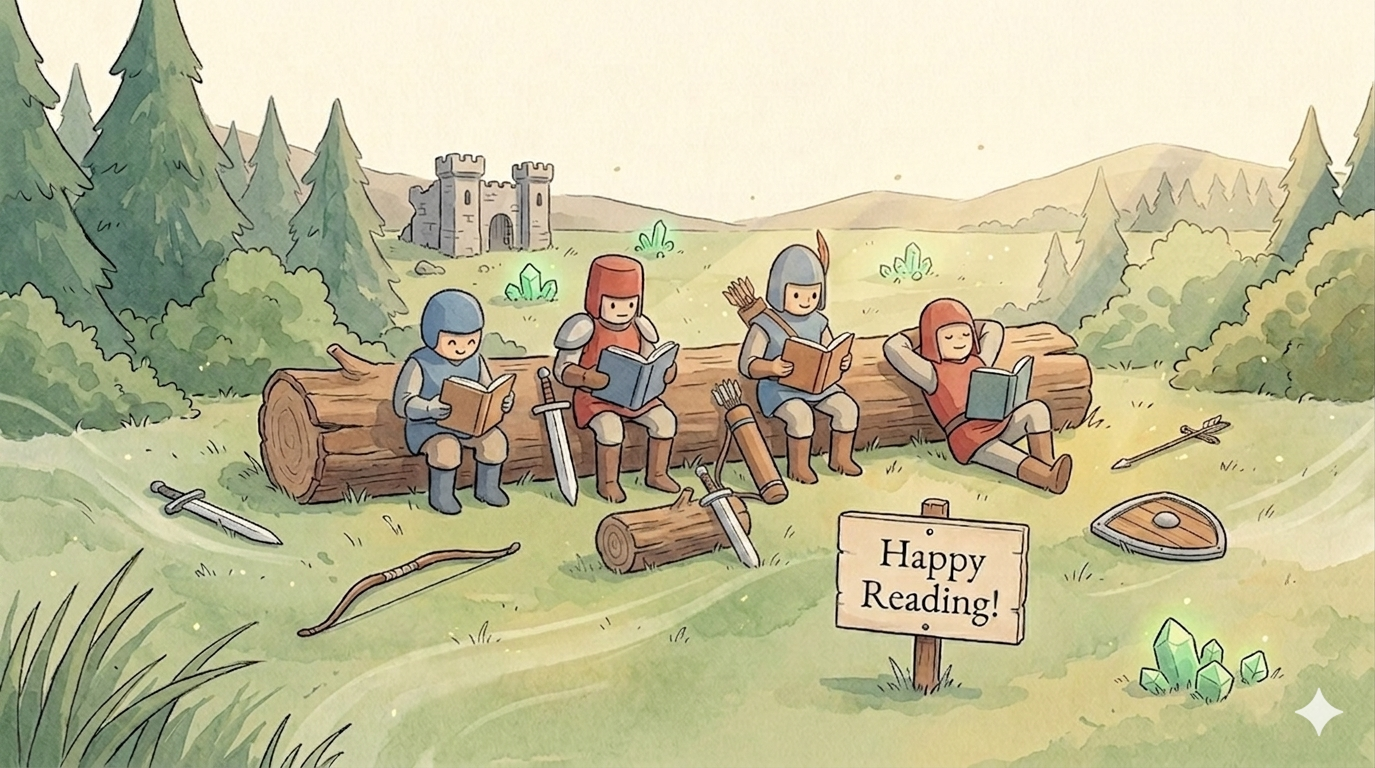
\includegraphics[width=0.98\linewidth]{chapters/00_interlude/figures/happy_reading.png}}%
        };
        \fill[happyCorner] 
            ([xshift=-0.9cm]img.south east) -- 
            ([xshift=-0.9cm, yshift=0.9cm]img.south east) -- 
            ([yshift=0.9cm]img.south east) -- cycle;
        \fill[white] 
            ([xshift=-0.9cm]img.south east) -- 
            (img.south east) -- 
            ([yshift=0.9cm]img.south east) -- cycle;
    \end{tikzpicture}
    
    \vspace{0.05cm}

    \begin{tikzpicture}
        \node[inner sep=0] (img) {%
            \setlength{\fboxrule}{2pt}\setlength{\fboxsep}{0pt}%
            \fcolorbox{endlessFrame}{white}{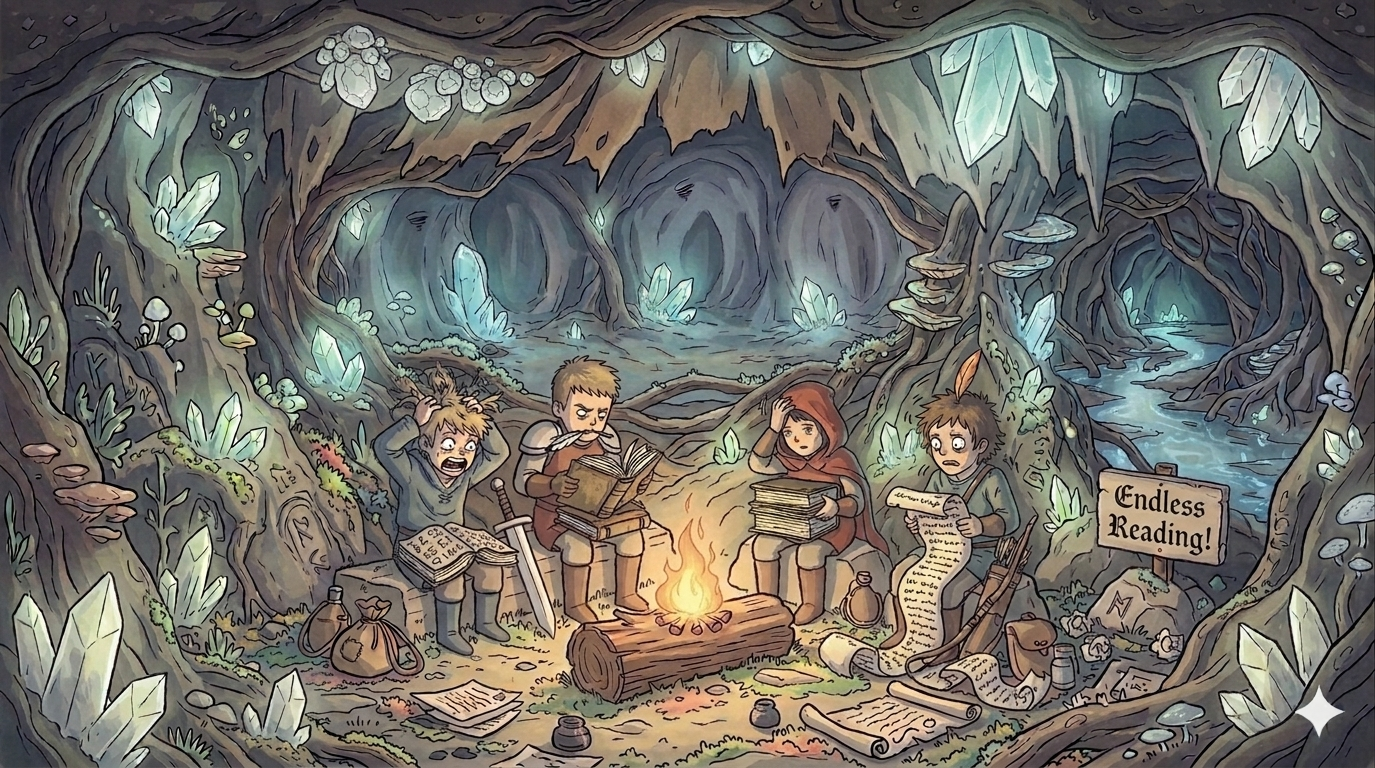
\includegraphics[width=0.98\linewidth]{chapters/00_interlude/figures/endless_reading.png}}%
        };
        \fill[endlessCorner] 
            ([xshift=-0.9cm]img.south east) -- 
            ([xshift=-0.9cm, yshift=0.9cm]img.south east) -- 
            ([yshift=0.9cm]img.south east) -- cycle;
        \fill[white] 
            ([xshift=-0.9cm]img.south east) -- 
            (img.south east) -- 
            ([yshift=0.9cm]img.south east) -- cycle;
    \end{tikzpicture}\\
    
    {\textit{``Happy Reading!''} and \textit{``Endless Reading!''} illustrations generated with Google Gemini.}
\end{center}

\vspace*{\fill}
\cleardoublepage